\documentclass[
a4paper,
12pt, 
twoside]{scrbook}

\usepackage[italian]{babel}
\usepackage[utf8]{inputenc}

%----------------------------------------------------------------------------------- tikz
\usepackage{tikz}
%-----------------------------------------------------------------------------------


%----------------------------------------------------------------------------------- global
\usepackage{amsthm}               % Used for newtheorem etc
\usepackage{graphicx}             % includegraphics 
\usepackage{amsfonts}             % An extended set of fonts for use in mathematics
\usepackage{amsmath}
\usepackage{amstext}
\usepackage{amssymb}
\usepackage{mathtools}            % Mathematical tools to use with amsmath
\usepackage{engrec}               % Convert number arguments to lower case or upper case greek letters
\usepackage{rotating}             % Let's rotate latex objects, even tables and captions
\usepackage{verbatim}             % Typesetting the contents of a file
\usepackage[safe,extra]{tipa}     % Fonts and macros for IPA phonetics characters
\usepackage{lmodern}
% \usepackage{showkeys}
\usepackage{multirow}             % Create multiple rows tables and stuff
\usepackage{hyperref}             % To link urls
\usepackage{microtype}            % Micro-typographic extensions
\usepackage{enumerate}            % Enumerate with redefinable labels
\usepackage{enumitem}             % Control layout of itemize, enumerate, description
\usepackage{physics}              % Typesetting physic equations with brakets operator etc
\usepackage{braket}               % Brakets <> {} 
\usepackage{marginnote}           % Notes in the margin everywhere you want
\usepackage{cancel}               % Places lines to cancel characters (ex a*2/a)
\usepackage{polynom}              % Macros for manipulating polynomials
\usepackage{booktabs}             % Enhances the quality of tables
\usepackage{pdfpages}             % Simplifies the inclusion of external multi-page PDF documents in LATEX documents
\usepackage{pgfplots}
\usepackage{ragged2e}

%----------------------------------------------------------------------------------- 
\usepackage{fancyhdr}
\pagestyle{fancy}
\fancyhf{}
\fancyhead[LE,RO]{\thepage}
\fancyhead[RE]{\footnotesize\nouppercase{\leftmark}}
\fancyhead[LO]{\footnotesize\nouppercase{\leftmark}} % \rightmark to display section numbering 
                                                      % instead of chapter numbering
\setlength{\headheight}{14.5pt} % as requested by fan
\renewcommand{\headrulewidth}{0pt}
%-----------------------------------------------------------------------------------


%----------------------------------------------------------------------------------- Colored Boxes
\usepackage{setspace}               % for LINE SPACING
\usepackage{multicol}               % for MULTICOLUMNS
\usepackage[many]{tcolorbox}    	% for COLORED BOXES (tikz and xcolor included)
\usepackage{xcolor}
\definecolor{main}{HTML}{5989cf}    % setting main color to be used
\definecolor{sub}{HTML}{cde4ff}     % setting sub color to be used
\setlength\parindent{0pt}           % killing indentation for all the text
\setstretch{1.4}                    % setting line spacing to 1.3
\setlength\columnsep{0.25in}        % setting length of column separator
\tcbset{
	sharp corners,
	colback = white,
	before skip = 0.2cm,            % add extra space before the box
	after skip = 0.5cm,             % add extra space after the box
	halign upper=justify
}           
%-----------------------------------------------------------------------------------

%----------------------------------------------------------------------------------- Equation font
\usepackage{unicode-math}           % Required to use math fonts
\setmathfont{TeX Gyre Bonum Math}   % Custom font for equations
%-----------------------------------------------------------------------------------

%----------------------------------------------------------------------------------- Fonts
\usepackage{titling}
\usepackage{fontspec}
\usepackage{titlesec}
\titleformat{\chapter}[display]
{\normalfont\ttfamily\huge\bfseries\color{black}}
{\chaptertitlename\ \thechapter}{20pt}{\Huge}
\titleformat{\section}
{\normalfont\ttfamily\Large\bfseries\color{black}}
{\thesection}{1em}{}
\titleformat{\paragraph}
{\normalfont\ttfamily\Large\bfseries\color{black}}
{\thesection}{1em}{}
%----------------------------------------------------------------------------------- Front page
\title{Appunti di Strade e Bim (Esercizi)}
\author{Università degli Studi di Napoli Federico II\\\ Ivano D'Apice\\\href{https://t.me/sonoivano}{@telegram}}
\date{}          
%-----------------------------------------------------------------------------------
          
\pgfplotsset{compat=1.13}           % based on tikz, compat gives compatibility

%-----------------------------------------------------------------------------------
\usepackage[modulo]{lineno}              % The 'modulo' option shows only line numbers multiple of 5
\preto{\chapter}{\resetlinenumber}       % 
%\linenumbers                             % Make line number of paragraphs
\newenvironment{chapquote}[2][2em]
{\setlength{\@tempdima}{#1}%
	\def\chapquote@author{#2}%
	\parshape 1 \@tempdima \dimexpr\textwidth-2\@tempdima\relax%
	\itshape}
{\par\normalfont\hfill--\ \chapquote@author\hspace*{\@tempdima}\par\vspace{4em}}
\makeatother
%-----------------------------------------------------------------------------------




%-----------------------------------------------------------------------------------
\begin{document}
	\fontfamily{lmtt}\selectfont                                       % typewriter font for the pdf
	\maketitle                                                         % Front page generation
	\setlist{leftmargin = 2cm}
%-----------------------------------------------------------------------------------


%-----------------------------------------------------------------------------------
    \renewcommand{\chaptermark}[1]{%
    	\markboth{\chaptername
    		\ \thechapter.\ #1}{}}
    \renewcommand{\sectionmark}[1]{\markright{\thesection.\ #1}}
    \newcommand{\floor}[1]{\lfloor #1 \rfloor}
    \newcommand{\MYhref}[3][blue]{\href{#2}{\color{#1}{#3}}}%
%-----------------------------------------------------------------------------------	

%-----------------------------------------------------------------------------------
	\newtcolorbox{boxK}{
		sharpish corners, % better drop shadow
		boxrule = 0pt,
		toprule = 4.5pt, % top rule weight
		enhanced,
		fuzzy shadow = {0pt}{-2pt}{-0.5pt}{0.5pt}{black!35} % {xshift}{yshift}{offset}{step}{options}
	}
	
	\newtcolorbox{boxF}{
		colback = sub,
		enhanced,
		boxrule = 1.5pt, 
		colframe = white, % making the base for dash line
		borderline = {1.5pt}{0pt}{main, dashed} % add "dashed" for dashed line
	}
%-----------------------------------------------------------------------------------	


%-----------------------------------------------------------------------------------
    \def\tagform@#1{\maketag@@@{\bfseries(\ignorespaces\textbf{#1}\unskip\@@italiccorr)}}
    \renewcommand{\eqref}[1]{\textup{{\normalfont(\ref{\textbf{#1}}}\normalfont)}}
%-----------------------------------------------------------------------------------


	\chapter*{Introduzione}
	\textbf{Questi appunti sono presi a lezione. Per quanto sia stata fatta
		una revisione è altamente probabile (praticamente certo) che possano
		contenere errori, sia di stampa che di vero e proprio contenuto. Per
		eventuali proposte di correzione inviare mail a: }
	\url{ivanodapice@hotmail.com}.\\
	
	\tableofcontents
	\chapter{Formulario I}
	\pagenumbering{roman} % Starts numbering page in lowercase roman numbers
    \section{Esercizio 1}
	{
	 \centering
	  \begin{tabular}{|c|c|c|c|} 
		\hline
		\rule[-1ex]{0pt}{2.5ex}  Autocarro & m=18t & Pa=60\% & Ne=120kW \\
		\hline
	  \end{tabular}\par
    }
    
    \leavevmode\newline
    
    \begin{boxK}
    	Determinare lo \textbf{sforzo di trazione} per mantenere una velocità \textbf{costante} di 55 Km/h su di un tronco stradale \textbf{rettilineo}, con pavimentazione \textbf{asciutta} con manto stradale con \textbf{micro e macrotessitura ed elementi a spigoli vivi}, ed in \textbf{salita} con la pendenza longitudinale i = 2\%. Verificare e indicare se lo \textbf{sforzo di trazione} calcolato è effettivamente \textbf{disponibile} ed \textbf{esplicabile}. 
    \end{boxK}
    
    \begin{equation}\label{eq:trazione}
    	T=P(\mu+\mu_{c}\pm i\pm \frac{\beta}{g}\frac{dv}{dt})+k\cdot S\cdot V^{2}
    \end{equation}
    
    \begin{boxF}
    	Dato che la strada in esame è in rettilineo, $\mu_{c}$=0. Inoltre, a velocità costante possiamo trascurare la componente di accelerazione $\frac{dv}{dt}$, e infine, $i$ avrà segno positivo perché in salita. L'equazione diventa:
    \end{boxF}
    
    \begin{equation}\label{eq:trazione2}
    	T=P(\mu+i)+k\cdot S\cdot V^{2}
    \end{equation}
    
    \leavevmode\newline
    
    {
     \centering
     \resizebox{\columnwidth}{!}{%
     \begin{tabular}{|c|c|}
     	\hline
     	$\mu$ & = 0,025. Valore dalla tabella 1 per V=20km/h (Dato che 55 è più vicino a 20 che a 100) \\
     	\hline
     	P     & = m$\cdot$g = 18000kg$\cdot$9,81m/s\texttwosuperior = 176580N\\
     	\hline
     	k     & = 0,025. Valore dalla tabella 1 per autocarri e autobus\\
     	\hline
     	S     & = 3,0. Valore dalla tabella 1 per autocarri e autobus\\
     	\hline
     \end{tabular}
    }
    
    \begin{equation}
    	T=176580(0,025+0,020)+0,025\cdot 3,0\cdot 55^{2}=8172,98N
    \end{equation}
    
    \begin{boxF}
    	Per verificare se lo sforzo di trazione sia esplicabile, poniamo $T\leq T_{esp}$ e cioè $T\leq Pa\cdot Fa$. Invece, per quanto riguarda la trazione disponibile, si pone come verifica $T\leq T_{dsp}=T\leq \frac{N_e\cdot 3,6}{V}$
    \end{boxF}
    \leavevmode\newline
    {
    	\centering
    	\resizebox{\columnwidth}{!}{%
    		\begin{tabular}{|c|c|}
    			\hline
    			Pa     & = 60\%P = 0,60$\cdot$P = 105948N\\
    			\hline
    			Fa     & = 0,45. Valore dalla tabella 4, curva 5, a velocità di 55km/h\\
    			\hline
    		\end{tabular}
    	}
    	
    \begin{equation}
    	T_{esp}=f_{a}\cdot P_{a}= 0,45\cdot 105948N= 47676,60N
    \end{equation}
    
    \begin{equation}
    	T_{disp}=\frac{N_e\cdot 3,6}{V}=\frac{120kW\cdot 3,6}{55km/h}=7,85kN=7850N
    \end{equation}
    
    \begin{equation}
    	T\leq T_{esp}\phantom{...}\textbullet\textnormal{Soddisfatto}\phantom{.....} T\leq T_{disp}\phantom{...}\circ\textnormal{Non Soddisfatto}
    \end{equation}
    \leavevmode\newline
    \leavevmode\newline
    \section{Esercizio 2}
    \leavevmode\newline
    {
    	\centering
    	\begin{tabular}{|c|c|c|c|}
    		\hline
    		\rule[-1ex]{0pt}{2.5ex}  Autovettura & m=1,9t & Pa=75\% & Ne=70kW\% \\
    		\hline
    	\end{tabular}\par
    }
    \leavevmode\newline
    
    \begin{boxK}
    	Determinare lo sforzo di trazione necessario all’avviamento su di un tronco stradale \textbf{rettilineo}, con pavimentazione \textbf{bagnata} in \textbf{conglomerato bituminoso}, in \textbf{salita} con la pendenza longitudinale i = 3,5\%, e con un’accelerazione confortevole a = dv/dt = 0,25 m/s\texttwosuperior. Verificare e indicare se lo sforzo di trazione calcolato è effettivamente \textbf{disponibile ed esplicabile}. 
    \end{boxK}
    
    \begin{equation}
    	T=P(\mu+\mu_{c}\pm i\pm \frac{\beta}{g}\frac{dv}{dt})+k\cdot S\cdot V^{2}
    \end{equation}
    
    \begin{boxF}
    	La componente $\mu_{c}$ si trascura sempre nel caso delle autovetture.\\
    	In avviamento, tralasciamo la parte relativa a $kSV^{2}$ e poniamo $V=5km/h$. 
    \end{boxF}
    
    {
    	\centering
    	\resizebox{\columnwidth}{!}{%
    		\begin{tabular}{|c|c|}
    			\hline
    			P     & = m$\cdot$g = 1900kg$\cdot$9,81m/s\texttwosuperior = 18639N\\
    			\hline
    			$\beta$     & = 1,05. Valore fissato\\
    			\hline
    			$\mu$     & = 0,020. Valore dalla tabella 1 preso per autovetture a 20km/h\\
    			\hline
    		\end{tabular}
    	}
    
    \begin{equation}
    	T=P(\mu+i+\frac{\beta}{g}\frac{dv}{dt})
    \end{equation}
    
    \begin{equation}
    	T=18639N(0,020+0,035+\frac{1,05}{9,81m/s^{s}}\cdot 0,25m/s^{2})=1523,90N
    \end{equation}
    \leavevmode\newline
    {
    	\centering
    	\resizebox{\columnwidth}{!}{%
    		\begin{tabular}{|c|c|}
    			\hline
    			Pa     & = 75\%P = 0,75$\cdot$P = 13979,25N\\
    			\hline
    			Fa     & = 0,50. Valore dalla tabella 4 in condizione di asciutto\\
    			\hline
    		\end{tabular}
    	}
    	
    	\begin{equation}
    		T_{esp}=f_{a}\cdot P_{a}= 0,50\cdot 13979,25N= 6989,63N
    	\end{equation}
    	
    	\begin{equation}
    		T_{disp}=\frac{N_e\cdot 3,6}{V}=\frac{70kW\cdot 3,6}{5km/h}=50,4kN=50400N
    	\end{equation}
    
    \begin{equation}
    	T\leq T_{esp}\phantom{...}\textbullet\textnormal{Soddisfatto}\phantom{.....} T\leq T_{disp}\phantom{...}\textbullet\textnormal{Soddisfatto}
    \end{equation}
    
    \section{Esercizio 3}
    \leavevmode\newline
    {
    	\centering
    	\begin{tabular}{|c|c|c|c|}
    		\hline
    		\rule[-1ex]{0pt}{2.5ex}  Autovettura & m=1,9t & Pa=80\% & Ne=50kW\% \\
    		\hline
    	\end{tabular}\par
    }
    
    \leavevmode\newline
    
    \begin{boxK}
    	Determinare la massima pendenza possibile di una strada tale che sia garantito l’\textbf{avviamento} in \textbf{salita} su un tronco stradale \textbf{rettilineo} con pavimentazione \textbf{asciutta} in \textbf{conglomerato bituminoso}. Si consideri un’accelerazione confortevole a = dv/dt = 0,30 m/s\texttwosuperior.
    \end{boxK}
     
    \leavevmode\newline
    
    \begin{equation}
    	T=P(\mu+i+\frac{\beta}{g}\frac{dv}{dt})
    \end{equation}
    
    \begin{equation}
    	\frac{T}{P}=\mu+i+\frac{\beta}{g}\frac{dv}{dt}
    \end{equation}
    
    \begin{equation}\label{trazioneimax}
    	\frac{T}{P}-\mu-\frac{\beta}{g}\frac{dv}{dt}=i
    \end{equation}
    	
    {
    	\centering
    	\resizebox{\columnwidth}{!}{%
    		\begin{tabular}{|c|c|}
    			\hline
    			P      & =m$\cdot$g = 1900kg$\cdot$9,81m/s\texttwosuperior = 18639N\\
    			\hline
    			Pa     & = 80\%P = 0,80$\cdot$P = 18639,00N\\
    			\hline
    			Fa     & = 0,85. Valore dalla tabella 4 in condizione di asciutto\\
    			\hline
    			$\mu$  & = 0,02. Valore dalla tabella 1 preso per autovetture a 20km/h\\
    			\hline
    		\end{tabular}
    	}	
    
    \begin{equation}
    	T_{esp}=f_{a}\cdot P_{a}= 0,85\cdot 18639,00N= 12674,52N
    \end{equation}
    
    \begin{equation}
    	T_{disp}=\frac{N_e\cdot 3,6}{V}=\frac{50kW\cdot 3,6}{5km/h}=36,00kN=36000N
    \end{equation}
    
    \begin{boxF}
    	Prendiamo il valore più piccolo tra $T_{esp}$ e $T_{disp}$ ponendolo come valore della trazione nella equazione [\ref{trazioneimax}]
    \end{boxF}
    	
    \begin{equation}
    	i=\frac{12674,52N}{18639,00N}-0,020-\frac{1,05}{9,81m/s^2}\cdot 0,30m/s^2=63\%
    \end{equation}	
    \leavevmode\newline
    
    \section{Esercizio 4}
    \leavevmode\newline
    {
    	\centering
    	\begin{tabular}{|c|c|c|c|}
    		\hline
    		\rule[-1ex]{0pt}{2.5ex}  Autocarro & m=20t & Pa=60\% & Ne=130kW\% \\
    		\hline
    	\end{tabular}\par
    }
    
    \leavevmode\newline
    
    \begin{boxK}
    	Determinare la massima accelerazione all’\textbf{avviamento} su di un tronco stradale \textbf{rettilineo} in \textbf{salita} che ha la pendenza longitudinale i = 3\% su di una pavimentazione \textbf{asciutta} con manto stradale con solo \textbf{microtessitura ed elementi a spigoli vivi}.  
    \end{boxK}  	
    	
    \begin{equation}
    	T=P(\mu+i+\frac{\beta}{g}\frac{dv}{dt})
    \end{equation}
    
    \begin{equation}
    	\frac{T}{P}=\mu+i+\frac{\beta}{g}\frac{dv}{dt}
    \end{equation} 	
    	
    \begin{equation}
    	\frac{g}{\beta}(\frac{T}{P}-\mu-i)=\frac{dv}{dt}
    \end{equation} 		
    	
    {
    	\centering
    	\resizebox{\columnwidth}{!}{%
    		\begin{tabular}{|c|c|}
    			\hline
    			P      & =m$\cdot$g = 20000kg$\cdot$9,81m/s\texttwosuperior = 196200N\\
    			\hline
    			Pa     & = 60\%P = 0,60$\cdot$P = 117720,00N\\
    			\hline
    			Fa     & = 0,75. Valore dalla tabella 4 in condizione di asciutto\\
    			\hline
    			$\mu$  & = 0,025. Valore dalla tabella 1 preso per autovetture a 20km/h\\
    			\hline
    		\end{tabular}
    	}		
    	
    \begin{equation}
    	T_{esp}=f_{a}\cdot P_{a}= 0,75\cdot 117720,00N= 88290,00N
    \end{equation}
    
    \begin{equation}
    	T_{disp}=\frac{N_e\cdot 3,6}{V}=\frac{130kW\cdot 3,6}{5km/h}=93,60kN=93600N
    \end{equation}	
    	
    \begin{equation}
    	\frac{dv}{dt}=\frac{9,81m/s^2}{1,05}(\frac{88290,00N}{196200N}-0,025-0,30)=3,7m/s^2
    \end{equation} 	
    	
    \section{Esercizio 5}	
    
    \begin{boxK}
    	Determinare le distanze di visibilità per il cambio di corsia, il sorpasso su di una strada ad unica carreggiata di \textbf{tipo C} nell'ipotesi che essa sia percorsa in \textbf{salita} da una autovettura ad una velocità V = 100 Km/h.\\
    	A1) Determinare, altresì, la distanza di arresto nell’ipotesi che l’autovettura freni in 150m. \\
    	A2) Determinare, altresì, la distanza di arresto nell’ipotesi di pendenza longitudinale i = 5\%. 
    \end{boxK}  
    
    \begin{equation}
    	D_c=2,6\cdot V=260m
    \end{equation} 	
    
    \begin{equation}
    	D_a=v\cdot t_{pr}+s_f
    \end{equation} 	
    
    \begin{equation}
    	t_{pr}=2,8-0,01\cdot V=1,8s
    \end{equation} 	
    
    \begin{boxF}
    	27,8m/s perché come si vede anche nella formula, v è minuscolo. Quando troviamo questo tipo di notazione, la velocità è in metri al secondo.
    \end{boxF}
    
    \begin{equation}
    	D_a=27,8m/s\cdot 1,8s+150m=200m
    \end{equation} 	
    
    \begin{equation}
    	D_a=0,78\cdot 100-0,0028\cdot 10000+\frac{10000}{254(0,35+0,05)}
    \end{equation} 		
    	
   \chapter{Formulario II} 	
    	
   \section{Esercizio 1} 	
   {
   	\centering
   	\begin{tabular}{|c|c|c|c|}
   		\hline
   		\rule[-1ex]{0pt}{2.5ex}  Autovettura & P=6,50kN & Pa=85\% & Strada di tipo C1 \\
   		\hline
   	\end{tabular}\par
   }
   \leavevmode\newline
   \begin{boxK}
   	\begin{itemize}
   		\item Determinare il raggio minimo della curva circolare planimetrica per cui è garantito l’equilibrio allo sbandamento dei veicoli adottando i valori di aderenza trasversale forniti dal DM 5/11/2001; 
   		\item Determinare la velocità di percorrenza al limite dello sbandamento dell’autovettura nell'ipotesi di un valore del coefficiente di aderenza fa = 0,45 e di pendenza longitudinale i = 3,5\%; 
   		\item Determinare l’accelerazione trasversale non compensata e compensata per i quesiti a) e b). 
   	\end{itemize}
   \end{boxK}  
   
   \begin{equation}
   	\frac{V^2}{R}=127(q+f_t)\Rightarrow R=\frac{V^2}{127(q+f_t)}
   \end{equation} 		
   
   \begin{boxF}
   	Dato che ci troviamo in condizione di percorrere una strada di tipo C1, avremo come limiti inferiori e superiori rispettivamente 60 e 100km/h. In ordine per calcolare Rmin useremo il limite inferiore di 60km/h, mentre il valore di pendenza q sarà dato da tabella nel DM.6792 a pagina 60. Ft è preso da tabella 4 a seconda di velocità e tipologia di strada.
   \end{boxF}
 	   
   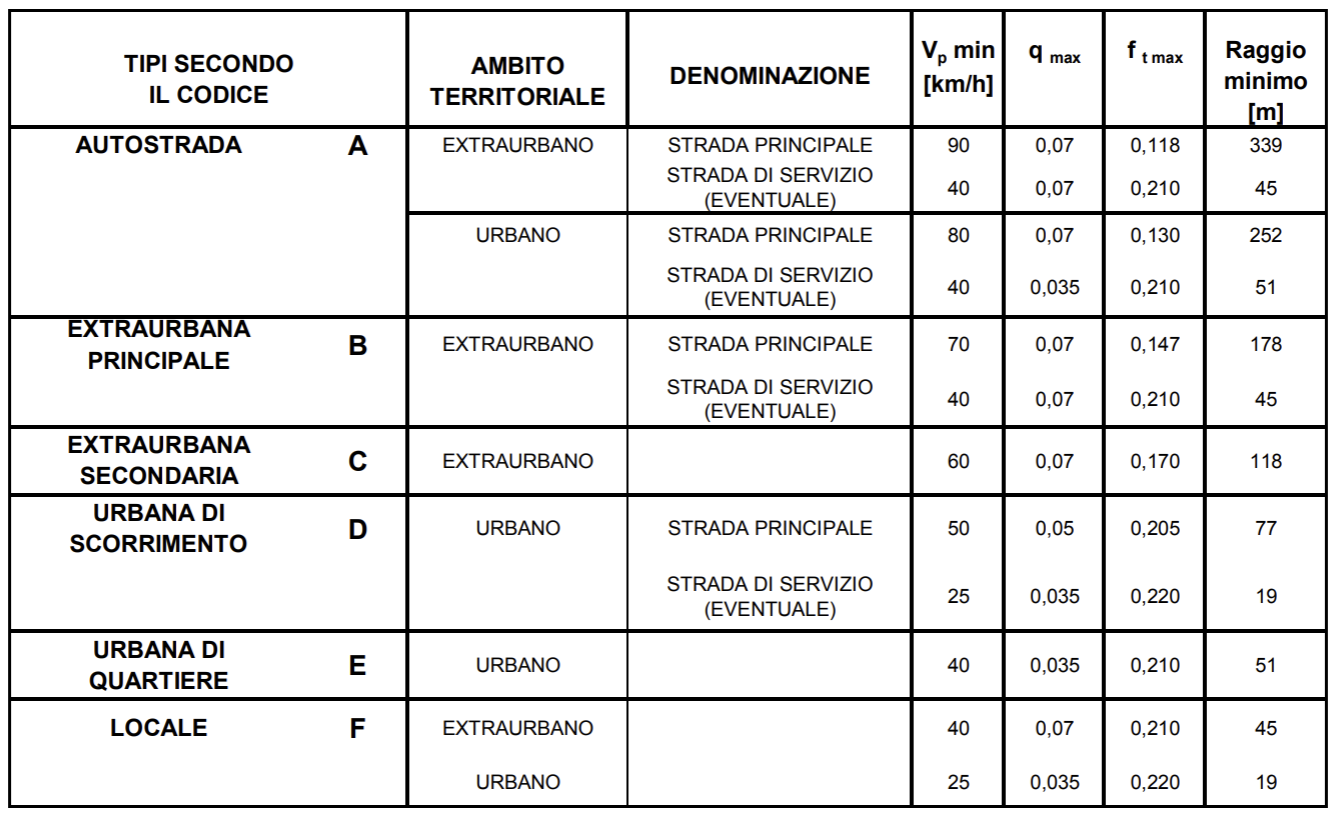
\includegraphics[width=\textwidth]{immagini/qmax.png} 	
    	
   \begin{equation}
   	R_{min}=\frac{60^2km^2/h^2}{127(0,07+0,17)}=118m
   \end{equation}
   
   \begin{equation}
   	V^2=127\cdot R(q+f_t)\Rightarrow V=\sqrt{127\cdot R(q+f_t)}
   \end{equation} 
    	
   \begin{boxF}
   	Ci troviamo in questa parte di progetto a verificare la velocità di percorrenza a limite di sbandamento. Ciò significa che ci troviamo nel caso limite in cui con tale velocità riusciamo ancora a rimanere su strada. Tale condizione viene data da T=A. Calcoleremo la velocità con la formula del raggio minimo interpolando Ft tramite trazione.
   \end{boxF} 	
   
   \begin{equation}
   	A=f_a\cdot P_a=\sqrt{f^{2}_l+f^{2}_t}\cdot P_a
   \end{equation} 
   
   {
   	\centering
   	\resizebox{\columnwidth}{!}{%
   		\begin{tabular}{|c|c|}
   			\hline
   			Pa     & = 85\%P = 0,85$\cdot$P = 5525,00N\\
   			\hline
   			K      & = 0,015. Valore dalla tabella 2 per autovetture di serie\\
   			\hline
   			$\mu$  & = 0,025. Valore dalla tabella 1 preso per autovetture a 100km/h\\
   			\hline
   			S      & = 1,50. Valore dalla tabella 3 per autovetture\\
   			\hline
   		\end{tabular}
   	}	
   	
   	\begin{equation}
   		T=P(\mu+i)\cdot K\cdot S\cdot V^2
   	\end{equation}
   	
   	\begin{equation}
   		T=6500N(0,025+0,035)+0,015\cdot 1,5m^2\cdot 60^2 km^2/h^2=471N
   	\end{equation}
   	
   	\begin{boxF}
   		Nelle componenti dell'aderenza trascuriamo quella trasversale riducendo tutto alla forza longitudinale.
   	\end{boxF} 	
   	
   	\begin{equation}
   		T=A=f_l\cdot P_a\Rightarrow f_l=\frac{T}{P_a}=\frac{471N}{5525N}=0,085
   	\end{equation}
   	
   	\begin{equation}
   		f_t=\sqrt{f^{2}_a-f^{2}_l}=\sqrt{0,45^2-0,085^2}=0,44
   	\end{equation}
   	
   	\begin{equation}
   		V=\sqrt{127\cdot 118m(0,07+0,44)}=87km/h
   	\end{equation}
   	
   	\begin{boxF}
   		Ricalcoliamo T con la nuova velocità per verificare che sia corretta.
   	\end{boxF} 	
   	
   	\begin{equation}
   		T=6500N(0,025+0,035)+0,015\cdot 1,5m^2\cdot 87^2 km^2/h^2=560N
   	\end{equation}
   	
   	\begin{equation}
   		f_l=\frac{T}{P_a}=\frac{560N}{5525N}=0,101
   	\end{equation}
   	
   	\begin{equation}
   		f_t=\sqrt{f^{2}_a-f^{2}_l}=\sqrt{0,45^2-0,101^2}=0,44
   	\end{equation}
   	
   	\begin{equation}
   		V=\sqrt{127\cdot 118m(0,07+0,44)}=87km/h
   	\end{equation}
   	
   	\begin{equation}
   		a_{nc1}=g\cdot f_t=9,81m/s^2\cdot 0,17=1,66m/s^2
   	\end{equation}
   	
   	\begin{equation}
   		a_{nc2}=g\cdot f_t=9,81m/s^2\cdot 0,44=4,32m/s^2
   	\end{equation}
   	
   	\begin{equation}
   		a_c=g\cdot q=9,81m/s^2\cdot 0,07=0,69m/s^2
   	\end{equation}
   	
   	\section{Esercizio 2}
    	
    \leavevmode\newline
    {
    	\centering
    	\begin{tabular}{|c|c|c|c|}
    		\hline
    		\rule[-1ex]{0pt}{2.5ex}  Autovettura & P=6,50kN & Pa=85\% & Strada di tipo C1 \\
    		\hline
    	\end{tabular}\par
    }
   \leavevmode\newline
   \begin{boxK}
   	\begin{itemize}
   		\item Determinare la pendenza trasversale q di una curva di raggio R = 750 m e la velocità di percorrenza V dell'autovettura secondo il DM 5/11/2001;  
   		\item Verificare se con il raggio assegnato è garantita la visibilità del ciglio interno. Si consideri per il calcolo del raggio che consente la visibilità del ciglio interno un valore di velocità pari a Vp,min. 
   	\end{itemize}
   \end{boxK}  
   
   \begin{equation}
   	R_{min}=\frac{60^2km^2/h^2}{127(0,07+0,17)}=118m
   \end{equation}
   
   \begin{equation}
   	R_{max}=\frac{100^2km^2/h^2}{127(0,07+0,11)}=437m
   \end{equation} 	
   
   \begin{equation}
   	R>R_{max}\Rightarrow V=V_{max}=100km/h
   \end{equation} 	
   
   {
   	\centering
   	\resizebox{\columnwidth}{!}{%
   		\begin{tabular}{|c|c|}
   			\hline
   			b     & = 1,23 da tabella 5, considerando la velocità \textbf{massima} per tipo di strada\\
   			\hline
   			$l_o$      & = 300m preso dall'abaco in figura 1 considerando la velocità \textbf{minima} per tipo di strada\\
   			\hline
   			$2\phi$  & = 78 gradi preso dall'abaco in figura 2 considerando la velocità \textbf{minima} per tipo di strada\\
   			\hline
   		\end{tabular}
   	}	
   
   \begin{equation}
    \ln q=-0,64\cdot \ln R+b
   \end{equation} 	
   
   \begin{equation}
   	\ln q=-0,64\cdot \ln 750m+1,23
   \end{equation} 	
   
   \begin{equation}
   	q=e^{-3}=0,5=5\%
   \end{equation} 	
   
   \begin{equation}
   	R_o=\frac{l_o}{sin(2\phi)}=\frac{300m}{sin(78\textdegree)}=306m
   \end{equation} 	
   
   \begin{equation}
   	R>R_o \Rightarrow \checkmark
   \end{equation} 	
   
   \section{Esercizio 3}
   {
   	\centering
   	\begin{tabular}{|c|c|c|c|}
   		\hline
   		\rule[-1ex]{0pt}{2.5ex}  Autovettura & P=6,50kN & Pa=85\% & Strada di tipo C1 \\
   		\hline
   	\end{tabular}\par
   }
   \begin{boxK}
   	Determinare la velocità di percorrenza V dell'autovettura e la pendenza trasversale q di una curva di raggio      R = 185 m secondo il DM 5/11/2001. 
   \end{boxK} 
    
   \begin{equation}
   	R_{min}<R<R_{max}\Rightarrow q=q_{max}=7\%=0,07
   \end{equation} 	
   
   \begin{boxF}
   	Calcoliamo V con l'equazione a Vmax per tipo di strada relativa a 100km/h, da risolvere come eq di secondo grado.
   \end{boxF}
   
   \begin{equation}
   	V^2(1-R\cdot0,0015)+V(R\cdot 0,432)-R\cdot 50,17=0
   \end{equation} 	
   
   \section{Esercizio 4}
   {
   	\centering
   	\begin{tabular}{|c|c|c|c|}
   		\hline
   		\rule[-1ex]{0pt}{2.5ex}  Autovettura & P=6,50kN & Pa=85\% & Strada di tipo C1 \\
   		\hline
   	\end{tabular}\par
   }
   \leavevmode\newline
   \begin{boxK}
   	Determinare per gli esercizi 2) e 3) nell'ipotesi di pendenza longitudinale i = 3.5\% e nell'ipotesi che osservatore ed ostacolo si trovino entrambi sulla curva circolare: 
   	\begin{itemize}
   	 \item la distanza minima D dell’asse della corsia da un ostacolo laterale, affinché sia garantita la distanza di visibilità nell’ipotesi di sorpasso e di arresto
   	 \item Il valore minimo del raggio R, affinché sia garantita la distanza di visibilità nell’ipotesi di sorpasso e di arresto. 
   	\end{itemize} 
   \end{boxK} 
   
   \begin{equation}
   	D=2\sqrt{2\cdot R\cdot \Delta}\Rightarrow \Delta=\frac{D^2}{8\cdot R}
   \end{equation} 	
   
   \begin{equation}
   	\begin{aligned}
   		D_S=5,5\cdot V\phantom{..............}\\
   		D_{S2}=5,5\cdot 100km/h=550m\\
   		D_{S3}=5,5\cdot 71km/h=390,5m
   	\end{aligned} 	
   \end{equation}
  
   \begin{equation}
   	\begin{aligned}
   		\Delta_{min,2}=\frac{550^2m^2}{8\cdot 750m}=50,4m\\
   		\Delta_{min,3}=\frac{390,5^2m^2}{8\cdot 185m}=103m
   	\end{aligned} 	
   \end{equation}
   
   \begin{equation}
   	D_A=0,78\cdot V-0,0028\cdot V^2+\frac{V^2}{254(f_e\pm i)}
   \end{equation} 	
   
   \begin{equation}
   	\begin{aligned}
   		D_{A2}=0,78\cdot 100km/h-0,0028\cdot 100^2km^2/h^2+\frac{100^2km^2/h^2}{254(0,35+0,035)}=156,26m\\
   		D_{A3}=0,78\cdot 71km/h-0,0028\cdot 71^2km^2/h^2+\frac{71^2km^2/h^2}{254(0,40+0,035)}=86,89m
   	\end{aligned} 	
   \end{equation}
   
   \begin{equation}
   	\begin{aligned}
   		\Delta_{min,2}=\frac{152,26^2m^2}{8\cdot 750m}=3,86m\\
   		\Delta_{min,3}=\frac{86,89^2m^2}{8\cdot 185m}=5,10m
   	\end{aligned} 	
   \end{equation}
   
   \begin{boxF}
   	Il valore di $\Delta$ per Rmin è dato dalla lunghezza della corsia più quello della banchina, tabellare da caratteristiche geometriche per tipo di strada
   \end{boxF}
   
   \begin{equation}
   	\begin{aligned}
   		R_{DS2,min}=\frac{D^2_{S2}}{8\cdot \Delta}=\frac{550^2m^2}{8\cdot 3,38m}=11187m\\
   		R_{DS3,min}=\frac{D^2_{S3}}{8\cdot \Delta}=\frac{390,5^2m^2}{8\cdot 3,38m}=5639,43m
   	\end{aligned} 	
   \end{equation}
   
   \begin{equation}
   	\begin{aligned}
   		R_{DA2,min}=\frac{D^2_{A2}}{8\cdot \Delta}=\frac{152,26^2m^2}{8\cdot 3,38m}=857,81m\\
   		R_{DA3,min}=\frac{D^2_{A3}}{8\cdot \Delta}=\frac{86,89^2m^2}{8\cdot 3,38m}=279,27m
   	\end{aligned} 	
   \end{equation}
   
   \chapter{Formulario III}
   
   \section{Esercizio 1}
   
   \begin{boxK}
   	Lo scostamento ∆R tra un rettifilo e una curva circolare di raggio R pari a 380m è 0,60m. La strada assegnata è di tipo C1 extraurbana.
   	\begin{itemize}
   		\item Determinare il parametro A della clotoide e verificare se tale parametro soddisfa i criteri indicati nel DM 5/11/2001; 
   		\item Determinare lo scostamento ∆R minimo che assicuri il superamento delle verifiche indicate nel D.M. 5/11/2001 per il parametro A della clotoide. Si trascuri per il calcolo di ∆R minimo la quantità $1+\frac{3}{14}\frac{\Delta R}{R}$;
   		\item Determinare le coordinate del centro del cerchio, le coordinate del punto finale e il valore di tc e rappresentare graficamente il raccordo rettifilo-clotoide-curva circolare indicando le grandezze fondamentali. 
   	\end{itemize}
   \end{boxK}  
   
   \begin{equation}
   	A=\sqrt[4]{24\cdot R^3\cdot \Delta R(1+\frac{3}{14}\frac{\Delta R}{R})}
   \end{equation} 	
   
   \begin{equation}
   	A=\sqrt[4]{24\cdot 380^3m^3\cdot 0,60m(1+\frac{3}{14}\frac{0,60m}{380m})}=167,67m
   \end{equation} 	
   
   \begin{equation}
   	A\geq A_{min,1}=0,021\cdot V^2
   \end{equation} 	
   
   \begin{equation}
   	R_{min}=\frac{60^2km^2/h^2}{127(0,07+0,17)}=118m
   \end{equation}
   
   \begin{equation}
   	R_{max}=\frac{100^2km^2/h^2}{127(0,07+0,11)}=437m
   \end{equation} 	
   
   \begin{equation}
   	R_{min}<R<R_{max} 
   \end{equation} 	
   
   \begin{boxF}
   	Dato che il raggio non può dirci il dato della velocità, lo ricaviamo tramite equazione di secondo grado
   \end{boxF}
   
   \begin{equation}
   	V^2(1-R\cdot0,0015)+V(R\cdot 0,432)-R\cdot 50,17=0
   \end{equation} 	
   
   \begin{equation}
   	V^2(0,43)+V(164,16)-19064,6=0
   \end{equation} 	
   
   \begin{equation}
   	V=\frac{-164,16\pm \sqrt{164,16^2-4(0,43\cdot -19064,6)}}{2\cdot 0,43}=93,32km/h
   \end{equation} 	
   
   \begin{equation}
   	A\geq A_{min,1}=0,021\cdot V^2=182m\phantom{////} \texttimes 
   \end{equation} 	
   
   \begin{equation}
   	A\geq A_{min,2}=\sqrt{\frac{R_f-R_i}{\Delta i_{max}}\cdot 100\cdot B(q_f+q_i)}
   \end{equation} 	
   
  \begin{boxF}
   $R_f$ è il raggio del cerchio che segue, mentre $R_i$ è quello che precede (rettifilo = 0). $q_f$ lo poniamo uguale a $q_{max}$ e $q_i$ a $q_{min}$. Nella formula per calcolare $\Delta i_{max}$ il valore di B è dato dalla distanza dell'asse di rotazione e ovvero dall'asse della corsia più la banchina.
  \end{boxF}
  
  \begin{equation}
  	\Delta i_{max}=\frac{18\cdot B_i}{V}
  \end{equation} 	
   
  \begin{equation}
  	A\geq A_{min,2}=\sqrt{\frac{380m}{\frac{18\cdot 5,25m}{93,32km/h}}\cdot 100\cdot 5,25m(0,07+0,025)}=136,8m\phantom{//} \checkmark
  \end{equation} 	
  
  \begin{equation}
  	A\geq A_{min,3}=\frac{R}{3}\phantom{//} \checkmark
  \end{equation} 	
  
  \begin{equation}
  	A\geq A_{min,4}=R\phantom{//} \checkmark
  \end{equation} 	
  
  \begin{equation}
  	A=\sqrt[4]{24\cdot 380^3m^3\cdot 0,60m(1+\frac{3}{14}\frac{0,60m}{380m})}
  \end{equation} 	
  
  \begin{equation}
  	A^4=24\cdot R^3\cdot \Delta R
  \end{equation} 	
  
  \begin{boxF}
  	Utilizziamo A=182,88m perché nella verifica è stato il valore non soddisfatto. Prendendolo ora per le successive verifiche sappiamo che è il valore minimo per cui tutte e 4 le prove sono soddisfatte.
  \end{boxF}
  
  \begin{equation}
  	\Delta R=\frac{A^4}{24\cdot R^3}=\frac{182,88^4m^4}{24\cdot 380^3m^3}=0,84m
  \end{equation} 	
  
  \begin{equation}
  	l=\frac{L}{A}=\frac{A^2}{R\cdot A}=\frac{A}{R}=\frac{182,88m}{380m}=0,48
  \end{equation} 	
  
  \begin{boxF}
  	Con questo valore di l andiamo a prendere tutte le componenti cartesiane che ci servono per disegnare la figura dalla tabella in fondo al formulario.
  \end{boxF}
  
  {
  	\centering
  	{%
  		\begin{tabular}{|c|c|}
  			\hline
  			$\tau_c$   & = 7,33\\
  			\hline
  			$x$        & = 0,4974m\texttimes A = 57,67m\\
  			\hline
  			$y$        & = 0,0184m\texttimes A = 3,36m\phantom{1} \\
  			\hline
  			$x_m$      & = 0,2399m\texttimes A = 43,87m\\
  			\hline
  			$y_m$      & = $R+\Delta R$ = 380m+0,84m = 80,84m\\
  			\hline
  		\end{tabular}
  	}	
  
    \section{Esercizio 2}
  
    \begin{boxK}
    	In figura sono assegnati due elementi curvilinei circolari di raggio R1 = 500m e R2 = 350m distanti D = 10m. Il verso di percorrenza è indicato. La strada assegnata è di tipo F1 extraurbana. 
    	\begin{itemize}
    		\item Determinare il parametro della clotoide di flesso e verificare se tale parametro soddisfa i criteri indicati nel DM 5/11/2001; 
    		\item Determinare le coordinate del centro dei cerchi, le coordinate dei punti iniziali e finali e i valori di $\tau_c$; 
    		\item Rappresentare graficamente il raccordo curva circolare-clotoide-curva circolare indicando tutte le grandezze fondamentali.
    	\end{itemize}
    \end{boxK}
    
    \begin{boxF}
    	Calcoliamo i valori relativi agli assi x e y della figura 2 del formulario.
    \end{boxF}
    
    \begin{equation}
    	\frac{R_2}{R_1}=0,7m
    \end{equation}
    
    \begin{equation}
    	\frac{D}{R_1}=0,02m
    \end{equation}
    
    \begin{boxF}
    	Grazie ai due dati precedenti possiamo prendere il valore della prossima frazione da tabella:
    \end{boxF}
    
    \begin{equation}
    	\begin{aligned}
    		\frac{A}{R_1}=0,43m\\
    		A=0,43m\cdot R_1=215m
    	\end{aligned} 	
    \end{equation}
   
    \begin{equation}
    	R_{min}=\frac{40^2km^2/h^2}{127(0,07+0,21)}=45m
    \end{equation}
    
    \begin{equation}
    	R_{max}=\frac{100^2km^2/h^2}{127(0,07+0,11)}=437m
    \end{equation} 	
    
    \begin{equation}
    	R>R_{max}\Rightarrow V=V_{max}=100km/h
    \end{equation} 	
    
    \begin{equation}
    	A\geq A_{min,1}=0,021\cdot V^2=210m\phantom{////} \checkmark
    \end{equation} 	
    
    \begin{equation}
    	A\geq A_{min,2}=\sqrt{\frac{R_f-R_i}{\Delta i_{max}}\cdot 100\cdot B(q_f+q_i)}
    \end{equation} 	
    
    \begin{boxF}
    	In questo caso possiamo trascurare B e $q_i$ la calcoliamo con l'equazione logaritmica.
    \end{boxF}
    
    \begin{equation}
    	A\geq A_{min,2}=\sqrt{\frac{500-350m}{18}\cdot V\cdot 100(0,064+0,07)}=105,71m\phantom{//} \checkmark
    \end{equation} 	
    
    \begin{equation}
    	A\geq A_{min,3}=\frac{R}{3}\phantom{//} \checkmark
    \end{equation} 	
    
    \begin{equation}
    	A\geq A_{min,4}=R\phantom{//} \checkmark
    \end{equation} 	
    
    \begin{equation}
    	A_1=A_2=215m
    \end{equation} 	
    
    \begin{equation}
    	l_1=\frac{215m}{500m}=0,43
    \end{equation} 	
    
    \begin{equation}
    	l_2=\frac{215m}{350m}=0,61
    \end{equation}
     	
    \leavevmode\newline
    
    {
    	\centering
    	{%
    		\begin{tabular}{|c|c|}
    			\hline
    			$\tau_{c1}$   & = 5,88\\
    			\hline
    			$x_1$         & = 0,4296m\texttimes A = 92,36m\\
    			\hline
    			$y_1$         & = 0,0132m\texttimes A = 2,84m\phantom{1} \\
    			\hline
    			$x_{m1}$      & = 0,2149m\texttimes A = 46,20m\\
    			\hline
    			$y_{m1}$      & = $R+\Delta R$ = 500m+0,7095m = 500,71m\\
    			\hline
    		\end{tabular}
    	}	
    \leavevmode\newline
    \leavevmode\newline
    \leavevmode\newline
    {
    	\centering
    	{%
    		\begin{tabular}{|c|c|}
    			\hline
    			$\tau_{c2}$   & = 11,84\\
    			\hline
    			$x_2$         & = 0,6079m\texttimes A = 130,70m\\
    			\hline
    			$y_2$         & = 0,0377m\texttimes A = 8,11m\phantom{1} \\
    			\hline
    			$x_{m2}$      & = 0,3046m\texttimes A = 65,49m\\
    			\hline
    			$y_{m2}$      & = $R+\Delta R$ = 350m+2,021m = 352,02m\\
    			\hline
    		\end{tabular}
    	}	
    
    \begin{equation}
    	\varepsilon=\arctan(\frac{x_{m1}+x_{m2}}{y_{m1}+y_{m2}})=7,46\textdegree
    \end{equation}
    
    \section{Esercizio 3}
    
    \begin{boxK}
    	Sono assegnate due livellette, la prima con pendenza $i_1$=-4,5\% e la seconda con pendenza $i_2$=+3,5\%. L’elemento che sottende il raccordo è una curva circolare di raggio R = 590m. La strada assegnata è di tipo B extraurbana principale.  
    	\begin{itemize}
    		\item Determinare il raggio e la lunghezza del raccordo verticale secondo i criteri indicati nel                  DM 5/11/2001. Si effettui il calcolo per D = Da;
    		\item Determinare le coordinate del vertice, del punto a tangenza orizzontale e il valore della freccia;  
    		\item Rappresentare graficamente il raccordo verticale indicando tutte le grandezze fondamentali
    	\end{itemize}
    \end{boxK}
    
    \begin{boxF}
    	Dato che abbiamo prima una discesa e poi una salita ($i_1=-, i_2=+$), la curva che si andrà a formare sarà concava.
    \end{boxF}
    
    \begin{equation}
    	\Delta i= i_2-i_1= 3,5\%-(-4,5\%)= 8,0\%= 0,08
    \end{equation}
    
     \begin{equation}
    	R_{min}=\frac{70^2km^2/h^2}{127(0,07+0,15)}=175m
    \end{equation}
    
    \begin{equation}
    	R_{max}=\frac{120^2km^2/h^2}{127(0,07+0,10)}=667m
    \end{equation} 	
    
    \begin{equation}
    	R_{min}<R<R_{max}
    \end{equation} 	
    
    \begin{equation}
    	V^2(1-R\cdot0,0015)+V(R\cdot 0,432)-R\cdot 50,17=0 \Rightarrow V=110km/h
    \end{equation} 	
    
    \begin{boxF}
    	Entriamo nell'abaco di figura 1 con pendenza longitudinale e velocità e ricaviamo la distanza di arresto. Con questa distanza poi vediamo in che zona degli abachi in figura 3 o 4 ci troviamo (D>L o D<L). In questo caso Da=170m e ci troviamo nella situazione di D<L.
    \end{boxF}
    
    \begin{equation}
    	L=\frac{\Delta i\cdot D^2_a}{2(h+D_a\cdot \vartheta)}
    \end{equation} 	
    
    \begin{boxF}
    	h è fissato a 0,5m mentre $\vartheta$ a 1 grado e ovvero 0,017 radianti.
    \end{boxF}
    
    \begin{equation}
    	L=\frac{0,08\cdot 170^2m^2}{2(0,5m+170m+0,017)}=341m
    \end{equation} 	
    
    \begin{equation}
    	L=\frac{D^2_a}{2(h+D_a\cdot \vartheta)}=4262,5m
    \end{equation} 	
    
    {
    	\centering
    	{%
    		\begin{tabular}{|c|c|}
    			\hline
    			$x_v$         & = $\frac{L}{2}$=170,5m\\
    			\hline
    			$x_a$         & = $-\frac{i_1}{\Delta i}\cdot L$=191,81m\\
    			\hline
    			$y_v$         & = $\frac{L\cdot i}{2}$=-7,67m \\
    			\hline
    			$y_a$         & = $-\frac{i^2_1}{2\Delta i}\cdot L$= -4,32m\\
    			\hline
    			$f$           & = $\left|\frac{\Delta i}{2L}\right|(\frac{L}{2})^2$ = 3,41m\\
    			\hline
    			$y_f$         & = $y_v-f$= -4,26m\\
    			\hline
    		\end{tabular}
    	}	
   
%
%%
%%%
%%%%
%%%%%
%%%%%%
%%%%%%%
%%%%%%%%
%%%%%%%%%
%%%%%%%%%%
%%%%%%%%%%%
%%%%%%%%%%%%
%%%%%%%%%%%%%
%%%%%%%%%%%%%%
\end{document}